\chapter{Cloud Service Ontology}
\label{cha:cocoon}
IaaS providers include Amazon Web Services (AWS), Microsoft Azure, Google, Alibaba and others. They give users the option to deploy their application over a pool of virtually infinite services with practically no capital investment and with modest operating costs proportional to the actual use. Elasticity, cost benefits and abundance of resources motivate many organizations to migrate their enterprise applications (e.g. Content management system, Customer relationship management system and Enterprise resource planning system) to the Cloud. Although Cloud offers the opportunity to focus on revenue growth and innovation, decision makers (e.g., CIOs, scientists, developers, engineers, etc.) are faced with the complexity of choosing among private, public, and hybrid Cloud options and selecting the right service delivery and deployment model, see Section \ref{sec:research_problem}.

To address this IaaS service discovery problem
we present an OWL-based ontology, the Cloud Computing Ontology (CoCoOn)
that defines functional and non-functional concepts, attributes
and relations of infrastructure services.

From a service discovery point of view, the selection process on the IaaS layer is based on a finite set of functional (e.g. CPU type, memory size, location) and non-functional (costs, QoS, security) configuration properties that can be satisfied by multiple providers. Similarly, there is a service discovery problem associated with the SaaS and PaaS offerings. However, we are not considering these issues in this thesis.
In cloud computing, SaaS services are often developed
and provided by third party service providers who are different from the IaaS providers.
We focus on IaaS that is the underpinning layer
on which the PaaS services are hosted for creating SaaS applications.
As there are less studies in IaaS selection compare to SaaS selection,
which a lot of the Service Composition techniques are directly applicable.


Although popular search engines (e.g., Google, Bing, etc)
can point users to these provider web sites (blogs, wikis, etc.)
that describe laaS service offerings, they are not designed to
compare and reason about the relations among the different
types of Cloud services and their configurations. Service
description models and discovery mechanisms for
determining the similarity among Cloud infrastructure
services are needed to aid the user in the discovery and
selection of the most cost effective infrastructure service
meeting the user's functional and non-functional
requirements.

In this chapter, We identify and formalize the domain knowledge of multiple
configurations of infrastructure services. The core idea is to
formally capture the domain knowledge of services using
semantic Web languages like the Resource Description
Framework (RDF) and the Web Ontology Language (OWL).
The contributions are as the following:
Identification of the most important concepts and
relations of functional and non-functional
configuration parameters of infrastructure services
and their definition in an ontology;
Modeling of service descriptions published by
Cloud providers according to the developed
ontology. By doing so, we validate the
expressiveness of ontology against the most
commonly available infrastructure services
including Amazon, Microsoft Azure, GoGrid, etc.


\section{Common Approaches}
In relation to research problem described in Section \ref{sec:research_problem}, there are 3 common approaches for web services identification/publication: 
\begin{enumerate}
    \item Manually maintain directories by categorizing manually-submitted or collected information about Cloud services and providers, an example of such kind is Universal Description, Discovery and Integration (UDDI), which has failed to gain wide adoption.
    \item Use web crawling, and automatically create listings.
    \item Combine both, e.g. using manually-submitted URIs as seeds to generate indexes. The first approach is the only feasible solution at the moment. But extensive research and standardization efforts have been put into developing web information representation models, namely, RDF, the semantic web, and ontologies \cite{Al-Hamdani2003}.
\end{enumerate}

\section{CoCoOn 0.1.0}
\label{sec:cocoon0.1}
The initial version of CoCoOn defines the
domain model of the IaaS layer. This ontology facilitates the
description of Cloud infrastructure services; and through
mappings from provider descriptions, facilitates the
discovery of infrastructure services based on their
functionality.
The ontology is defined in the OWL \cite{OWL}.
To describe specific aspects of
Cloud computing, established domain classifications have
been used as a guiding reference
\cite{UnifiedOntologyCloudComputing}.
For the layering of the ontology on top of Web service models,
it draws inspiration and ideas from standard semantic Web service ontologies i.e.,
OWL-S \cite{BringingSemanticsToWebServicesOWL-S}
and WSMO \cite{WSMO}. Consequently, modelers can use the
grounding model and process model of OWL-S in
combination with the presented Cloud computing ontology
to succinctly express common infrastructure Cloud services.
We mapped the most prominent set of infrastructure services
(i.e. Amazon, Azure, GoGrid, Rackspace, etc.) to CoCoOn.
All common meta data fields in the ontology including
Organization, Author, First Name etc. are referenced through
standard Web Ontologies (i.e. FOAF \cite{FOAF} and
Dublin Core \cite{DublinCore}).

The first version of CoCoOn consists of two parts:
functional Cloud service configurations information
parameters; and non-functional service configuration
parameters. In the following sections, we detail on these two
parts. We also present parts of the ontology in a visual form
produced by the Cmap Ontology Editor tool \cite{CmapToolsOntologyEditor}.

\subsection{Functional Parameters}
The main concept to describe functional Cloud service
configurations in CoCoOn 0.1.0 is a CloudResource that can be of
one of the three types: Infrastructure-as-a-Service ,
Platform-as-a-Service or Software-as-a-Service.

Cloud services in the IaaS layer can be categorised into:
Compute, Network, and Storage services
(See Fig. \ref{fig:CoCoOn0.1CloudResource}).
Compute is the main concept for infrastructure services,
whereas Network and Storage are usually attached to a
Compute service (with exceptions, for example
NetworkStorage).
Due to page limit, a larger graph is made available online at
\href{https://cmapscloud.ihmc.us/viewer/cmap/1SB4SYXQ2-1NW70FR-1MMSKJ}{here}.
The previous model's graph was generated by Cmap \cite{cmap}. 

\begin{figure}
  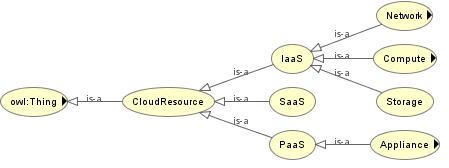
\includegraphics[width=\textwidth,keepaspectratio]{Figures/0.1/CloudResource.png}
  \caption{CoCoOn 0.1.0 Top Concepts in the IaaS layer}
  \label{fig:CoCoOn0.1CloudResource}
\end{figure}

The Compute class (see Fig. \ref{fig:CoCoOn0.1SubClassesPropertiesComputeStorageNetwork}) has the following object properties, hasVirtualization, hasCPU, hasMemoryAddressSize and hasNetworkStorage. The hasCPU property links a Compute unit to one or many processors which can be of type CPU or ClusteredCPU. A Compute object can be linked to a Storage object by using the top level object property hasStorage.

\begin{figure}
  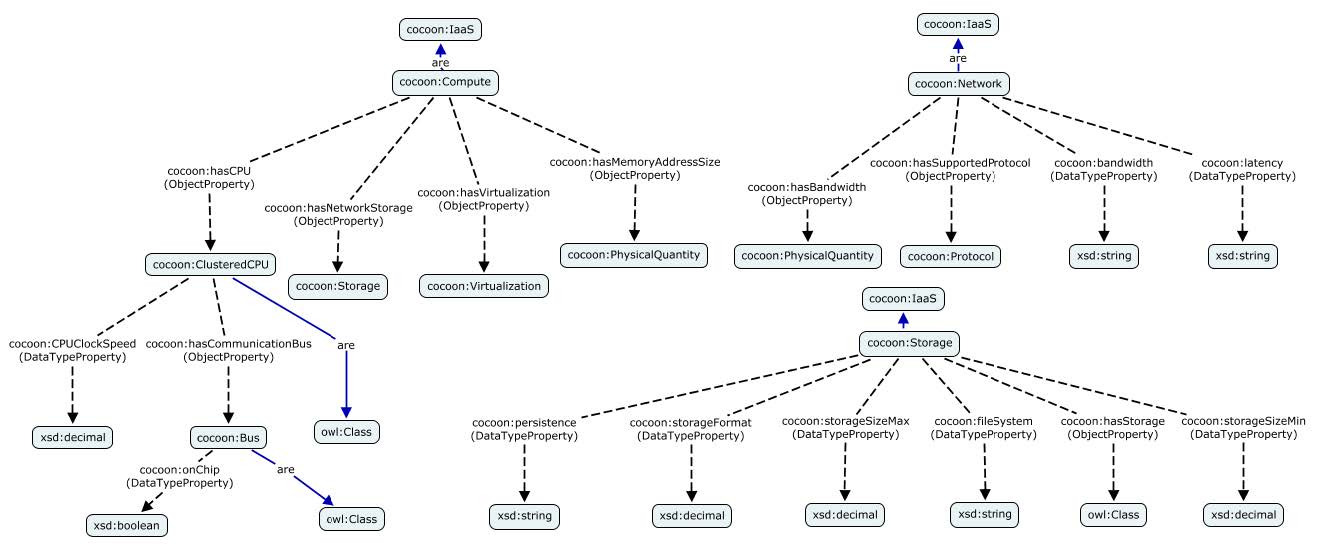
\includegraphics[width=\textwidth,keepaspectratio]
  {Figures/0.1/SubClassesPropertiesComputeStorageNetwork.jpg}
  \caption{CoCoOn 0.1.0 SubClasses and properties for the Compute, Storage and Network class}
  \label{fig:CoCoOn0.1SubClassesPropertiesComputeStorageNetwork}
\end{figure}

There are two different Storage types for a CloudResource: LocalStorage attached to a CPU with the hasLocalStorage property and NetworkStorage attached to a Compute instance with the hasNetworkStorage property. The hasNetworkStorage is an \textit{owl:inverseOf} property of the isAttached property which can be used to define that a Storage resource is attached to a Compute resource. There is also an important distinction to be made between Storage resources that \underline{are} attached to a Compute resource and Storage resources that \underline{can be} attached. The latter is modeled with the \textit{isAttachable} object property and its inverse property \textit{hasAttachable}. These relations are important for the discovery of infrastructure services based on a user requirement.
For example, in the case of Amazon, we can model that a \textit{BlockStorage} with a \textit{StorageSizeMin} of 1GB and a \textit{StorageSizeMax} of 1TB can be attached to any EC2 Compute resource instance i.e., Standard, Micro, High-Memory, High-CPUCluster, ComputeCluster, GPUHigh-I/O.
Consequently, if a user searches for a specific Compute instance with, for example, 5GB persistent storage, the relevant EC2 Compute resource and an Amazon BlockStorage will be returned (possibly among others). That is, because the isAttached relation in the user request can be matched with the definition of the Amazon EC2 unit with a BlockStorage defined to be isAttachable.

A Network resource can be described with the
has Bandwidth and hasProtocol properties. Similarly, to how
Storage resources are attached to Compute resource, we
distinguish between the hasSupportedNetwork and
hasNetwork property to either express that the specific
network types can be used with a Compute resource or that
they are in fact used.

\subsection{Non-Functional Parameters}
For non-functional Cloud service configuration parameters we distinguish between non-functional properties and QoS attributes. The first are properties of Cloud resources that are known at design time, for example,
PriceStorage, Provider, DeploymentModel,
whereas QoS attributes can only be recorded after at least one execution cycle of a Cloud service, for example, DiskReadOperations, Networkln, NetworkOut etc.
For QoS attributes, we distinguish MeasurableAttributes like the ones above and
UnmeasurableAttributes like Durability or Performance.

The QoS attributes define a taxonomy of Attributes and Metrics,
i.e. two trees formed using the \textit{rdfs:subClassOf} relation where
a ConfigurationParameter, for example, PriceStorage, PriceCompute, PriceDataTransferIn (Out) etc;
and a Metric, for example, ProbabilityOfFailureOnDemand, TransactionalThroughput, are used in combination to
define non-functional properties (e.g. Performance, Cost, etc.). The resulting ontology is a directed graph where, for example,
the Property hasMetric (and its inverse isMetricOf) is the basic link between ConfigurationParameters and \textit{Metric} trees. For the
QoS metrics, we used existing QoS ontologies \cite{QoSOnt} as a reference whereas
for the ConfigurationParameters concepts the ontology defines its independent taxonomy, but refer to external ontologies for existing definitions
(e.g. QUDT \cite{QUDT}). Each configuration
parameter has a \textit{Name} and a \textit{Metric} (qualitative or quantitative).
The \textit{Metric} itself has UnitOfMeasurement and Value. The type of configuration determines the nature of a service by means of setting a minimum, maximum, or capacity limit, or meeting a certain value. For example, the hasMemory configuration parameter
of a Compute service can be set to have a Value of 2 and a UnitOfMeasurement of GB.

\section{CoCoOn 1.0.1}
\label{sec:cocoon1.0.1}
As the Web brings people into an age of information overload,
presenting only most relevant personalized and reliable
information to customers is crucial to business success.
Consumers of Cloud computing services also need better recommendation
for them to make informed decisions.
To fulfill the goal of a smart Cloud service recommendation,
an unified model is needed as foundation for data collection reasoning and analytics.
Due to the Cloud's relative new emergence compared to traditional Computer Science fields, there is a lack of a well recognized standard ontology model.
Semantic technologies are commonly employed to build such a model.
Since there are other models that focus on such a model for Services and Web Services in general, our model only focuses on Cloud computing Infrastructure as a Services (IaaS) aspects like features and prices.

The ontology can be accessed online via:
\url{https://w3id.org/cocoon/v1.0.1}

\subsection{Major Change}
We have proposed a simpler model describing concepts of Cloud infrastructure services (IaaS)
in our previous work \cite{IJNGC2013,CoCoOn2012},
see Section \ref{sec:cocoon0.1}. This work was mostly a taxonomy of IaaS.
In this section we will propose an extension focusing on the core parameters for comparing and recommending IaaS services.

We also aware of the popularity of schema.org, and hence made this version compatible with its vocabularies and hope CoCoOn can become an extension to schema.org, as there is no existing definition covered the Cloud service domain. During this process we observed that despite schema.org's wide deployments among websites, it is not defined with OWL2 semantics, which has the most expressive power (in comparison to RDF).

We revised our CoCoOn ontology, i.e. changes have been made to namespaces, classes, properties, relationships and axioms, with a strong focus on flexibility and extensibility.

We also introduced versioning from this release, for both ontology and data, following the
\href{https://semver.org/}{semantic versioning specification}. Although this ontology is not in a sense of "in production",
this version is a stable release that we are intended to keep long term support and availability. We label the collection date of data with \schema{dateModified}, thus historical price data can be recorded.

The new model is outlined in Section \ref{sec:CoCoOnextended},
with explanation of its syntax and semantics, design, formalization.

It has been a long time since we proposed the initial model of CoCoOn, which we retrospectively versioned 0.1.0, hence there are many advances in both the Semantic Web field and Cloud Computing.
The major model changes are summarized below:
\begin{enumerate}
  \item Additional external vocabularies.
  \item Additional annotations, including version number, modification dates, metadata like author,
  web page etc.
  \item Removed classes and properties which are not core, and possibly covered by some other ontologies, e.g. Input, Output, Interface, User.
  \item New class and properties focusing on IaaS and price specifications. Like \cocoon{CloudOSPriceSpecification} and various other extensions to \gr{UnitPriceSpecification}; subclasses for specific Cloud features i.e. \cocoon{LoadBalancing}; classes for describing properties like \cocoon{TrafficDirection}, which specifies network data flow direction.
\end{enumerate}
A detailed change log can also be find on the online documentation 
\href{https://w3id.org/cocoon/v1.0.1#changes}{"Changes from last version" section}.

On top of that we developed a full mapping service between CoCoOn 1.0.1, and Cloud vendor APIs for the Google Cloud and the Microsoft Azure Cloud.
These mapping services demonstrates the usability and strength of the ontology developed. More details can be found in Section \ref{sec:cocoonImplementation}.

We also used existing ontologies whenever fits, such as 
the Unit of Measure Ontology (QUDT) \cite{OntologyUnitsOfMeasure} for defining price with currency values, see Section \ref{sec:ReusingExistingVocabularies} for more details.

\subsection{Reusing Existing Vocabularies}
\label{sec:ReusingExistingVocabularies}
A set of well-known vocabularies has evolved in the Semantic Web community.
The set of established vocabularies we reuse are listed in Table \ref{table:namespaces}.

\begin{longtable}[ht]{ p{.15\textwidth} p{.35\textwidth} |p{.15\textwidth} p{.25\textwidth} }
\hline
Names & Details & Namespaces & URIs \\ \hline
OWL2 & Web Ontology Language Schema 2. & owl & \url{http://www.w3.org/2002/07/owl\#} \\ \hline
RDF & Resource Description Framework Concepts Vocabulary. & rdf & \url{http://www.w3.org/1999/02/22-rdf-syntax-ns\#}\\
& RDF Schema vocabulary. & rdfs & \url{http://www.w3.org/2000/01/rdf-schema\#} \\
\hline
XML Schema Definition & Data types for elements and attributes. & xsd & \url{http://www.w3.org/2001/XMLSchema\#} \\ \hline
DCMI Metadata Terms & Defines general metadata attributes. & dcterms & \url{http://purl.org/dc/terms/}\\ \hline
VANN & Vocabulary for annotating descriptions of vocabularies with examples and usage notes. & vann & \url{http://purl.org/vocab/vann/} \\ \hline
Friend of a Friend & People and relationship. & foaf & \url{http://xmlns.com/foaf/0.1/} \\ \hline
Creative Commons & License terms. & cc & \url{http://creativecommons.org/ns\#}  \\ \hline
Geo Names & Geographic places. & gn & \url{http://www.geonames.org/ontology\#} \\ \hline
Schema.org & Vocabulary for common concepts, i.e. TypeAndQuantityNode, GeoCoordinates, e.t.c. & schema & \url{https://schema.org/} \\ \hline
Good Relations & Product, price and company data. & gr & \url{http://purl.org/goodrelations/v1\#} \\\hline
QUDT & Units and measurements schema. & qudt & \url{http://qudt.org/schema/qudt\#}\\ 
& Unit vocabulary. & unit & \url{http://qudt.org/vocab/unit\#}\\
\hline
Semantic Sensor Network & SSN is an ontology for describing sensors and their observations, the studied features of interest, the samples used to do so, and the observed properties. & ssn & \url{http://www.w3.org/ns/ssn/}\\
& System capabilities terms of SSN ontology. & ssn-system & \url{http://www.w3.org/ns/ssn/systems/}\\
& Sample Observation and Actuator. & sosa & \url{http://www.w3.org/ns/sosa/}\\
\hline
\caption{Vocabularies}
\label{table:namespaces}
\end{longtable}

We have also considered a number of other vocabularies, but decided they are not suitable for our case:
\begin{enumerate}
  \item OWL-S \cite{OWL-S}: It is more useful when defining the input, output and interactions between web services, but CoCoOn is not modeling those.
  \item Unified Code for Units of Measure (UCUM) \cite{UCUM} and Custom Datatypes \cite{CDT}: These ontologies do not include the units needed for our use case, see Section \ref{sec:unit}.
\end{enumerate}

\subsection{Concepts and Design}
\label{sec:CoCoOnextended}
The relevant code and ontology itself is made available online at this
\href{https://github.com/miranda-zhang/cloud-computing-schema}{Github project page}.

In this section we describe the main conceptual components of CoCoOn 1.0.1,
how they evolved, the rationale behind their design and some example usages.
The examples are in Turtle syntax \cite{turtle}. 
The class expressions are in
\href{http://protegeproject.github.io/protege/class-expression-syntax/}{Manchester OWL Syntax}
\cite{ManchesterOWLSyntax},
which is what Protege \cite{Protege} use.
We will show the prefix definitions once,
then omit the duplicated definitions in the following examples.

The specification of the models suggests the arrangement of classes and properties according to subsumption hierarchies
(OWL uses the \rdfs{subClassOf} for representing subsumption),
which represent the skeleton of the model and establish the basic relationships between the components.

Following the principle of minimal commitment \cite{principles_for_minimal_commitments},
we use guarded restriction (i.e., existential quantifier, $\exists$,
\magenta{some}, \owl{someValuesFrom})
instead of domain range restrictions (\rdfs{domain}, \rdfs{range}).
As such, the domain and ranges are more permissive,
keeping the model more flexible.
We also use qualified cardinality restrictions
(e.g., \magenta{exactly}, \owl{qualifiedCardinality};
\magenta{max}, \owl{maxQualifiedCardinality}) when there
is a known cardinality restriction.

\subsubsection{Cloud Service Feature}
Most building blocks of IaaS services naturally correspond to OWL2 classes 
(e.g., \cocoon{CloudService}, \cocoon{ComputeService}, \cocoon{StorageService}), object properties (e.g., \cocoon{hasMemory}, \cocoon{hasStorage}, \cocoon{inRegion})
and data properties (e.g., \cocoon{numberOfCores}).
The more challenging part is to capture constraints posed by the possible combination of services in IaaS in the models using ontological axioms.
We next describe how this was accomplished using a combination of OWL2 axioms and integrity constraints.

\subsubsubsection{Cloud Service}
The class \cocoon{CloudService} is the main class hosting our Cloud feature vocabularies.
We defined a top level class \cocoon{Service} to be its parent, and make it the union of \schema{Service} and \sosa{FeatureOfInterest}.
So our Cloud service definitions are compatible with schema.org and SOSA ontology.
As later we need to use vocabularies from both.

Cloud Services are usually classified into three categories:
\cocoon{IaaS}, \cocoon{PaaS}, \cocoon{SaaS}.
We focus on modelling IaaS, see Section \ref{sec:IaaS} for more details.
We have classified \cocoon{SystemImage} as a subclass of \cocoon{SaaS},
as a computer system is like any other software, and can be installed on different compatible hardware.
Some examples of \cocoon{SaaS} are database as a service, machine learning as a service, Google Cloud Composer, etc.
Some examples of \cocoon{PaaS} are Google App Engine, Heroku, etc.

The following properties are defined for the class \cocoon{CloudService}:
\begin{itemize}
    \item[] \gr{hasPriceSpecification} \magenta{some} \gr{UnitPriceSpecification}
    \item[] \cocoon{hasProvider} \magenta{exactly} 1 \gr{BusinessEntity}
    \item[] \cocoon{inRegion} \magenta{exactly} 1 \cocoon{Region}
    \item[] \cocoon{inZone} \magenta{max} 1 \xsd{string}
\end{itemize}

We use \gr{UnitPriceSpecification} and its associated object property \gr{hasPriceSpecification}
to model price, see Section \ref{sec:PriceSpecification} for more details about price specification.
Existential quantifiers (i.e., \magenta{some}, \owl{someValuesFrom}) are used on \gr{hasPriceSpecification}.

Note that, \magenta{some} is the same as \magenta{min} 1. 
But this is not the same as database integrity constrains.
We can still define (Cloud service) individuals without a price specification.
Under the open world assumption, missing information is just not known but may exist, whereas in databases (closed world assumption), absence of information often assumes that the information does not exist.
We can not guarantee all services will have a price specification, as there are services available upon request, but the price is negotiated later. For example, we may want to specify that secure data centers for governmental use
are available, but detailed information is probably not disclosed publicly.

We assume each service can belong to exactly one provider.
A qualified cardinality restriction \magenta{exactly} (\owl{qualifiedCardinality}) is used to define this type of assumption.
We used \gr{BusinessEntity} to describe a provider, see Section \ref{sec:Provider} for more details.

\subsubsubsection{Infrastructure as a Service}
\label{sec:IaaS}
Infrastructure as a Service can be classified into 3 categories:
\cocoon{ComputeService} (see Section \ref{sec:VM}),
\cocoon{StorageService} (see Section \ref{sec:Storage}),
\cocoon{NetworkService} (see Section \ref{sec:Network}).

\subsubsubsection{Compute Service}
\label{sec:VM}
We define the following properties for class \cocoon{ComputeService}:
\begin{itemize}
  \item[] \cocoon{numberOfCores} \magenta{max} 1 \xsd{decimal}
  \item[] \cocoon{hasCPUcapacity} \magenta{max} 1 \schema{TypeAndQuantityNode}
  \item[] \cocoon{hasMemory} \magenta{exactly} 1 \schema{TypeAndQuantityNode}
  \item[] \cocoon{hasStorage} \magenta{max} 1 \schema{TypeAndQuantityNode}
  \item[] \cocoon{hasMaxStorageSize} \magenta{max} 1 \schema{TypeAndQuantityNode}
  \item[] \cocoon{hasMaxNumberOfDisk} \magenta{max} 1 \schema{TypeAndQuantityNode}
  \item[] \gr{hasPriceSpecification} \magenta{max} 1 \cocoon{CloudStorageTransactionsPriceSpecification}
\end{itemize}

The number of cores available on a virtual machine(VM) is defined by the data property \cocoon{numberOfCores}.
Because it can have non integer value, we made it accept \xsd{decimal}.
For Google Cloud, cores and vCPU refer to the same thing.

\cocoon{hasCPUcapacity} is used to describe the performance power of the CPU.

The memory size of a VM is specified by \cocoon{hasMemory}.

The \cocoon{LocalStorage} available on a VM can be specified with \cocoon{hasStorage}.
We quantify this object property with \magenta{some}, so that it is possible to define more \cocoon{NetworkStorage} later.
Google has a limit for the maximum number of disks that can be attached to a VM, which we model with the object property \cocoon{hasMaxNumberOfDisk}.
Additionally, Google also has a limit for the maximum total disk size that can be attached to a VM, which is modelled with \cocoon{hasMaxStorageSize}.

We use \schema{TypeAndQuantityNode} to describe some quantity of things.
So value, unit, and the type of the object can all be captured. See Section \ref{sec:TypeAndQuantityNode} for more examples.

Note that this class also inherits properties from its super classes, e.g. the property inherited from \cocoon{CloudService}:

\gr{hasPriceSpecification} \magenta{some} \gr{UnitPriceSpecification}

We provids a short example of \cocoon{ComputeService} in Listing \ref{lst:VM}.

There are data access fees on local disk of the Azure VM \cite{data_access_fees_local_disk_AzureVM}. To model this we use
\gr{hasPriceSpecification} \magenta{max} 1 \cocoon{StorageTransactionsPriceSpecification}.
See Section \ref{sec:StorageTransactionsPriceSpecification} for an example.

\begin{lstlisting}[caption={Virtual Machine},label={lst:VM}]
@prefix schema: <https://schema.org/> .
@prefix unit:  <http://qudt.org/vocab/unit#> .
@prefix xsd:   <http://www.w3.org/2001/XMLSchema#> .
@prefix rdfs:  <http://www.w3.org/2000/01/rdf-schema#> .
@prefix gr:    <http://purl.org/goodrelations/v1#> .
@prefix cocoon: <https://w3id.org/cocoon/v1.0.1#> .
@base <https://w3id.org/cocoon/data/v1.0.1/> .
<2019-02-12/ComputeService/Gcloud/CP-COMPUTEENGINE-VMIMAGE-N1-HIGHCPU-96-PREEMPTIBLE>
        a                         cocoon:ComputeService ;
        rdfs:label                "CP-COMPUTEENGINE-VMIMAGE-N1-HIGHCPU-96-PREEMPTIBLE" ;
        gr:hasPriceSpecification  [ a                        cocoon:CloudServicePriceSpecification ;
                                    gr:hasCurrency           "USD" ;
                                    gr:hasCurrencyValue      "0.72"^^xsd:float ;
                                    gr:hasUnitOfMeasurement  unit:Hour ;
                                    cocoon:inRegion         <Region/Gcloud/us-east1>
                                  ] ;
        cocoon:hasMemory          [ a                        schema:TypeAndQuantityNode ;
                                    schema:amountOfThisGood  86.4 ;
                                    schema:unitCode          cocoon:GB
                                  ] ;
        cocoon:hasProvider        cocoon:Gcloud ;
        cocoon:numberOfCores      "96"^^xsd:decimal ;
        schema:dateModified       "2019-02-12"^^xsd:date .
<2019-03-07/ComputeService/Azure/windows-m128-64ms-standard>
        a                         cocoon:ComputeService ;
        rdfs:label                "windows-m128-64ms-standard" ;
        gr:hasPriceSpecification  <2019-03-07/CloudStorageTransactionsPriceSpecification/Azure/vm_base> ;
        gr:hasPriceSpecification  [ a                        cocoon:CloudServicePriceSpecification ;
                                    gr:hasCurrency           "USD" ;
                                    gr:hasCurrencyValue      "47.827e0"^^xsd:float ;
                                    gr:hasUnitOfMeasurement  unit:Hour ;
                                    cocoon:inRegion         <Region/Azure/japan-east>
                                  ] ;
        cocoon:hasMemory          [ a                        schema:TypeAndQuantityNode ;
                                    schema:amountOfThisGood  "3800"^^xsd:decimal ;
                                    schema:unitCode          cocoon:GB
                                  ] ;
        cocoon:hasProvider        cocoon:Azure ;
        cocoon:hasStorage         [ a                        schema:TypeAndQuantityNode ;
                                    schema:amountOfThisGood  "4096"^^xsd:decimal ;
                                    schema:typeOfGood        cocoon:LocalStorage ;
                                    schema:unitCode          cocoon:GB
                                  ] ;
        cocoon:numberOfCores      "64"^^xsd:decimal ;
        schema:dateModified       "2019-03-07"^^xsd:date .
\end{lstlisting}

\subsubsubsection{Storage Service}
\label{sec:Storage}
We define the following properties for the class \cocoon{StorageService}:
\begin{itemize}
  \item[] \cocoon{canHaveSnapshot} \magenta{some} \cocoon{StorageService}
  \item[] \cocoon{hasStorageIOMax} \magenta{max} 1 \schema{TypeAndQuantityNode}
  \item[] \cocoon{hasStorageSize} \magenta{max} 1 \schema{TypeAndQuantityNode}
  \item[] \cocoon{hasStorageThroughputMax} \magenta{max} 1 \schema{TypeAndQuantityNode}
\end{itemize}
Two subclasses of storage services have been defined: \cocoon{LocalStorage} and \cocoon{NetworkStorage}.

On Azure Cloud, snapshots options are available for storage, which is modeled with
the object property \cocoon{canHaveSnapshot}. This information is 
\href{https://github.com/miranda-zhang/cloud-computing-schema/blob/master/example/azure/storage.md#disk-snapshots}{manually interpreted from the documentation}.
There are also caps on input/output operations per sec (IOPS) and throughput, which are modeled with
\cocoon{hasStorageIOMax} and \cocoon{hasStorageThroughputMax}. We have also defined corresponding units, see Section \ref{sec:unit}.

In example Listing \ref{lst:Storage}, we have show a \cocoon{NetworkStorage} service from \cocoon{Azure}, which is a Cloud provider we have pre-defined as a named instance.
For more details on its corresponding Storage Transactions Prices,
see Section \ref{sec:StorageTransactionsPriceSpecification}.
Followed this we have given an example of snapshot service with only some of the regions shown. Next, the Azure provisional Ultra SSD storage service. It has configurable IOPS and throughput, and price are based on provisioned storage size, IOPS and throughput.This is also a reservation charge imposed if you enable Ultra SSD capability on the VM without connecting an Ultra SSD disk, which is rate at per vcpu/hour provisioned.

\begin{lstlisting}[caption={Storage},label={lst:Storage}]
@base <https://w3id.org/cocoon/data/v1.0.1/> .
<2019-03-07/NetworkStorage/Azure/premiumssd-p30>
        a                               cocoon:NetworkStorage ;
        rdfs:label                      "premiumssd-p30" ;
        gr:hasPriceSpecification        <CloudStorageTransactionsPriceSpecification/Azure/managed_disk/transactions-ssd> ;
        gr:hasPriceSpecification        [ a                        gr:CloudServicePriceSpecification ;
                                          gr:hasCurrency           "USD" ;
                                          gr:hasCurrencyValue      "135.17e0"^^xsd:float ;
                                          gr:hasUnitOfMeasurement  cocoon:GBPerMonth ;
                                          cocoon:inRegion         <Region/Azure/australia-east>
                                        ] ;
        cocoon:canHaveSnapshot          <NetworkStorage/Azure/standardssd-snapshot> , <NetworkStorage/Azure/standardhdd-snapshot-zrs> , <NetworkStorage/Azure/premiumssd-snapshot> , </NetworkStorage/Azure/standardhdd-snapshot-lrs> ;
        cocoon:hasProvider              cocoon:Azure ;
        cocoon:hasStorageIOMax          [ a                        schema:TypeAndQuantityNode ;
                                          schema:amountOfThisGood  "5000"^^xsd:nonNegativeInteger ;
                                          schema:unitCode          cocoon:IOPs
                                        ] ;
        cocoon:hasStorageSize           [ a                        schema:TypeAndQuantityNode ;
                                          schema:amountOfThisGood  "1024"^^xsd:nonNegativeInteger ;
                                          schema:unitCode          cocoon:GB
                                        ] ;
        cocoon:hasStorageThroughputMax  [ a                        schema:TypeAndQuantityNode ;
                                          schema:amountOfThisGood  "200"^^xsd:nonNegativeInteger ;
                                          schema:unitCode          unit:MegabitsPerSecond
                                        ].
<2019-03-07/NetworkStorage/Azure/standardssd-snapshot>
        a                         cocoon:NetworkStorage ;
        rdfs:label                "standardssd-snapshot" ;
        gr:hasPriceSpecification  [ a                        gr:CloudServicePriceSpecification ;
                                    gr:hasCurrency           "USD" ;
                                    gr:hasCurrencyValue      "0.1188e0"^^xsd:float ;
                                    gr:hasUnitOfMeasurement  cocoon:GBPerMonth ;
                                    cocoon:inRegion         <Region/Azure/south-india>
                                  ] ;
        gr:hasPriceSpecification  [ a                        gr:CloudServicePriceSpecification ;
                                    gr:hasCurrency           "USD" ;
                                    gr:hasCurrencyValue      "0.132e0"^^xsd:float ;
                                    gr:hasUnitOfMeasurement  cocoon:GBPerMonth ;
                                    cocoon:inRegion         <Region/Azure/canada-east>
                                  ] .
<2019-03-07/NetworkStorage/Azure/ultrassd>
        a                         cocoon:NetworkStorage ;
        rdfs:label                "ultrassd" ;
        gr:hasPriceSpecification  [ a                        gr:CloudServicePriceSpecification ;
                                    rdfs:label               "stored" ;
                                    gr:hasCurrency           "USD" ;
                                    gr:hasCurrencyValue      "8.2E-5"^^xsd:float ;
                                    gr:hasUnitOfMeasurement  cocoon:GBPerHour ;
                                    cocoon:inRegion         <Region/Azure/us-east-2>
                                  ] ;
        gr:hasPriceSpecification  [ a                        gr:CloudServicePriceSpecification ;
                                    rdfs:label               "iops" ;
                                    gr:hasCurrency           "USD" ;
                                    gr:hasCurrencyValue      "3.4E-5"^^xsd:float ;
                                    gr:hasUnitOfMeasurement  cocoon:IOPsPerHour ;
                                    cocoon:inRegion         <Region/Azure/us-east-2>
                                  ] ;
        gr:hasPriceSpecification  [ a                        gr:CloudServicePriceSpecification ;
                                    rdfs:label               "throughput" ;
                                    gr:hasCurrency           "USD" ;
                                    gr:hasCurrencyValue      "6.85E-4"^^xsd:float ;
                                    gr:hasUnitOfMeasurement  cocoon:MegabitsPerSecondPerHour ;
                                    cocoon:inRegion         <Region/Azure/us-east-2>
                                  ] ;
        gr:hasPriceSpecification  [ a                        gr:CloudServicePriceSpecification ;
                                    rdfs:label               "vcpu" ;
                                    gr:hasCurrency           "USD" ;
                                    gr:hasCurrencyValue      "0.003e0"^^xsd:float ;
                                    gr:hasUnitOfMeasurement  cocoon:VcpuPerHour ;
                                    cocoon:inRegion         <Region/Azure/us-east-2>
                                  ] .
<2019-02-12/NetworkStorage/Gcloud/CP-COMPUTEENGINE-STORAGE-PD-SSD-REGIONAL>
        a                         cocoon:NetworkStorage ;
        rdfs:label                "CP-COMPUTEENGINE-STORAGE-PD-SSD-REGIONAL" ;
        gr:hasPriceSpecification  [ a                        gr:CloudServicePriceSpecification ;
                                    gr:hasCurrency           "USD" ;
                                    gr:hasCurrencyValue      "0.29"^^xsd:double ;
                                    gr:hasUnitOfMeasurement  cocoon:GBPerMonth ;
                                    cocoon:inRegion         <Region/Gcloud/asia-south1>
                                  ] ;
        cocoon:hasProvider        cocoon:Gcloud ;
        schema:dateModified       "2019-02-12"^^xsd:date .
\end{lstlisting}

\subsubsubsection{Network Service}
\label{sec:Network}
We classify network services into the following categories:
\cocoon{InternetService}, \cocoon{LoadBalancing}, \cocoon{StaticIPService} and \cocoon{DNSService}.

\paragraph{Internet Service}
\label{sec:Internet}
We define the following properties for the class \cocoon{InternetService}:
\begin{itemize}
  \item[] \cocoon{hasDirection} \magenta{exactly} 1 \cocoon{TrafficDirection}
  \item[] \cocoon{hasDestination} \magenta{some} \cocoon{Location}
  \item[] \cocoon{excludesDestination} \magenta{some} \cocoon{Location}
\end{itemize}
There is generally no charge to ingress traffic,
unless there is a load balancer used.
We use the \cocoon{hasDirection} object property to indicate the direction of traffic.
A class \cocoon{TrafficDirection} is also constructed with 2 disjoint subclasses:
\cocoon{Egress} and \cocoon{Ingress}. Those can be used to indicate the direction of traffic.

Internet egress rates are based on usage and destination.
For example, Google Cloud has the following destination categories:
Australia, China (excluding Hong Kong) and
Worldwide (excluding China and Australia, but including Hong Kong).
In this case, the object properties \cocoon{hasDestination} and \cocoon{excludesDestination} can be used to specify destination ranges.
Because traffic destinations are not constrained by cloud service regions,
\cocoon{Location} is used, see Section \ref{sec:Region} for more details.

The internet egress traffic prices can be modeled by \cocoon{CloudNetworkPriceSpecification}, see Section \ref{sec:NetworkPriceSpecification} for more details.

Listing \ref{lst:GoogleCloudNetworkPriceWorldwide} shows an example for Google Cloud Internet Service Prices.

\begin{lstlisting}[caption={Google Cloud Network Price Example: Worldwide Egress},label={lst:GoogleCloudNetworkPriceWorldwide}]
@base <https://w3id.org/cocoon/data/v1.0.1/2019-02-12/> .
<InternetService/Gcloud/CP-COMPUTEENGINE-INTERNET-EGRESS-NA-NA>
        a                           cocoon:InternetService ;
        rdfs:label                  "CP-COMPUTEENGINE-INTERNET-EGRESS-NA-NA" ;
        gr:hasPriceSpecification    [ a                         cocoon:CloudNetworkPriceSpecification ;
                                      gr:hasCurrency            "USD" ;
                                      gr:hasCurrencyValue       "0.11"^^xsd:float ;
                                      gr:hasUnitOfMeasurement   cocoon:GBPerMonth ;
                                      cocoon:forUsageLessEqual  cocoon:10TB ;
                                      cocoon:forUsageMoreThan   cocoon:1TB
                                    ] ;
        gr:hasPriceSpecification    [ a                         cocoon:CloudNetworkPriceSpecification ;
                                      gr:hasCurrency            "USD" ;
                                      gr:hasCurrencyValue       "0.08"^^xsd:float ;
                                      gr:hasUnitOfMeasurement   cocoon:GBPerMonth ;
                                      cocoon:forUsageLessEqual  cocoon:90TB ;
                                      cocoon:forUsageMoreThan   cocoon:10TB
                                    ] ;
        gr:hasPriceSpecification    [ a                         cocoon:CloudNetworkPriceSpecification ;
                                      gr:hasCurrency            "USD" ;
                                      gr:hasCurrencyValue       "0.12"^^xsd:float ;
                                      gr:hasUnitOfMeasurement   cocoon:GBPerMonth ;
                                      cocoon:forUsageLessEqual  cocoon:1TB ;
                                      cocoon:forUsageMoreThan   [ a                        schema:TypeAndQuantityNode ;
                                                                  schema:amountOfThisGood  "0"^^xsd:nonNegativeInteger ;
                                                                  schema:unitCode          cocoon:GB
                                                                ]
                                    ] ;
        cocoon:excludesDestination  <Location/China> , <Location/Australia> ;
        cocoon:hasDestination       <Location/Worldwide> , <Hong%20Kong> ;
        cocoon:hasDirection         cocoon:Egress ;
        cocoon:hasProvider          cocoon:Gcloud ;
        schema:dateModified         "2019-02-12"^^xsd:date .
\end{lstlisting}

\paragraph{Load Balancing}
\label{sec:LoadBalancing}
Both hardware and software-based load balancing solutions exist. 
Here we consider load balancing as a hardware feature, unless it is known otherwise.
We create a class \cocoon{LoadBalancing} to represent such a service.
It is further broken down into 2 subclasses: \cocoon{LoadBalancingData} and
\cocoon{ForwardingRule}.

Ingress data processed by a load balancer is charged (Per GB) based on region.
Listing \ref{lst:LoadBalancingDataPriceSpecification} shows an example modelling such case with \cocoon{LoadBalancingData}.
\begin{lstlisting}[caption={Load Balancing Data Price Specification},label={lst:LoadBalancingDataPriceSpecification}]
@base <https://w3id.org/cocoon/data/v1.0.1/2019-02-12/> .
<LoadBalancingData/Gcloud>
        a                         cocoon:LoadBalancingData ;
        gr:hasPriceSpecification  [ a                        gr:CloudServicePriceSpecification ;
                                    gr:hasCurrency           "USD" ;
                                    gr:hasCurrencyValue      "0.008e0"^^xsd:float ;
                                    gr:hasUnitOfMeasurement  cocoon:GB ;
                                    cocoon:inRegion         <Region/Gcloud/us>
                                  ] ;
        gr:hasPriceSpecification  [ a                        gr:CloudServicePriceSpecification ;
                                    gr:hasCurrency           "USD" ;
                                    gr:hasCurrencyValue      "0.009e0"^^xsd:float ;
                                    gr:hasUnitOfMeasurement  cocoon:GB ;
                                    cocoon:inRegion         <Region/Gcloud/europe-west4>
                                  ] ;
        cocoon:hasDirection       cocoon:Ingress ;
        cocoon:hasProvider        cocoon:Gcloud ;
        schema:dateModified       "2019-02-12"^^xsd:date .
\end{lstlisting}

Forwarding rules that are created for load balancing are also charged.
This can be modelled by \cocoon{ForwardingRule}.
For example, pricing for rules on the Google Cloud:

\begin{displayquote}
Up to 5 forwarding rules are charged at 0.025 USD/hour. That means, if you create one forwarding rule, you will be charged 0.025/hour. If you have 3 forwarding rules, you will still be charged 0.025/hour.
However, if you have 10 rules, you will be charged:
\begin{itemize}
  \item[] 5 forwarding rules = 0.025/hour
  \item[] Each additional forwarding rule = 0.01/hour
  \item[] 0.025/hour for 5 rules + (5 additional rules * 0.01/hour) = 0.075/hour
\end{itemize}
\end{displayquote}

\cocoon{CloudNetworkPriceSpecification} can be used to model its price, see example Listing \ref{lst:LoadBalancingRulesPrice}.

\begin{lstlisting}[caption={Load Balancing Rules Price},label={lst:LoadBalancingRulesPrice}]
@base <https://w3id.org/cocoon/data/v1.0.1/> .
@prefix unit:  <http://qudt.org/1.1/vocab/unit#> .
<2019-02-12/ForwardingRule/Gcloud/base>
        a                         cocoon:ForwardingRule ;
        rdfs:comment              "Google Lord Balancing Forwarding Rule Base Rate. Flat rate price, regardless 1 rule or 5 rules used, charged the same per hour." ;
        rdfs:label                "FORWARDING_RULE_CHARGE_BASE" ;
        gr:hasPriceSpecification  [ a                         cocoon:CloudNetworkPriceSpecification ;
                                    gr:hasCurrency            "USD" ;
                                    gr:hasUnitOfMeasurement   unit:Hour ;
                                    cocoon:forUsageLessEqual  <TypeAndQuantityNode/5> ;
                                    cocoon:forUsageMoreThan   [ 
                                        a                        schema:TypeAndQuantityNode ;
                                        schema:amountOfThisGood  "0"^^xsd:nonNegativeInteger
                                                              ] ;
                                    cocoon:hasCurrencyValue   "0.038e0"^^xsd:float ;
                                    cocoon:inRegion          <Region/Gcloud/asia-northeast>
                                  ] ;
        cocoon:hasProvider        cocoon:Gcloud ;
        schema:dateModified       "2019-02-12"^^xsd:date .
<TypeAndQuantityNode/5>
        a                        schema:TypeAndQuantityNode ;
        schema:amountOfThisGood  "5"^^xsd:nonNegativeInteger .
\end{lstlisting}

\paragraph{Static IP Address}
The IP address of an VM instance usually does not guarantee to stay the same between
reboots/resets. So you may want to reserve a static external IP address for
your customers or users to rely on accessing the machine.
An example from Google: 
\begin{displayquote}
No charge for an IP address in use,
i.e. used it with a Compute Engine resource or a forwarding rule.
However, Google will charge 0.010 USD/Hour if you reserve a static external IP address but do not use it.
\end{displayquote}
This can be modelled with \cocoon{StaticIPService} and \cocoon{CloudServicePriceSpecification}.

\subsubsection{Cloud Service Price}
Regarding price modeling we extended vocabularies in GoodRelations.
GoodRelations is a Web Ontology Language-compliant ontology for Semantic Web online data, dealing with business-related goods and services. In November 2012, it was integrated into the \url{Schema.org} ontology.

\subsubsubsection{Cloud Service Price Specification}
\label{sec:PriceSpecification}
We defined \cocoon{CloudServicePriceSpecification} as a subclass of \gr{UnitPriceSpecification}.
One service can be offered in multiple regions, so we defined the property:

\cocoon{inRegion} \magenta{some} \cocoon{Region}

For more details on region, see Section \ref{sec:Region}.

In GoodRelations, there is a \gr{hasCurrencyValue} property taking a \xsd{float} as range.
However, sometimes we encountered values smaller than that, so we extended the existing class to allow double floating-point numbers (i.e. \xsd{double}):

\cocoon{hasCurrencyValue} \magenta{exactly} 1 (\xsd{double} or \xsd{float})

Listing \ref{lst:PriceSpecification} shows an example price specification for a Compute service from Azure. For more example usages see Section \ref{sec:IaaS} and \ref{sec:VM}.

\begin{lstlisting}[caption={Price Specification for Compute service from Azure},label={lst:PriceSpecification}]
@base <https://w3id.org/cocoon/data/v1.0.1/2019-03-07/> .
<ComputeService/Azure/linux-hc44rs-lowpriority>
        a                         cocoon:ComputeService ;
        rdfs:label                "linux-hc44rs-lowpriority" ;
        gr:hasPriceSpecification  <CloudStorageTransactionsPriceSpecification/Azure/vm_base> ;
        gr:hasPriceSpecification  [ a                        cocoon:CloudServicePriceSpecification ;
                                    gr:hasCurrency           "USD" ;
                                    gr:hasCurrencyValue      "0.317e0"^^xsd:float ;
                                    gr:hasUnitOfMeasurement  unit:Hour ;
                                    cocoon:inRegion          <Region/Azure/us-west-2>
                                  ] ;
        cocoon:hasMemory          [ a                        schema:TypeAndQuantityNode ;
                                    schema:amountOfThisGood  "352"^^xsd:decimal ;
                                    schema:unitCode          cocoon:GB
                                  ] ;
        cocoon:hasProvider        cocoon:Azure ;
        cocoon:hasStorage         [ a                        schema:TypeAndQuantityNode ;
                                    schema:amountOfThisGood  "700"^^xsd:decimal ;
                                    schema:typeOfGood        cocoon:LocalStorage ;
                                    schema:unitCode          cocoon:GB
                                  ] ;
        cocoon:numberOfCores      "44"^^xsd:decimal ;
        schema:dateModified       "2019-03-07"^^xsd:date .
\end{lstlisting}

We also defined specialized subclasses to handle the following scenarios:
the price of a VM image (\cocoon{CloudOSPriceSpecification}),
price of storage transactions (\cocoon{CloudStorageTransactionsPriceSpecification}),
and price of network services (\cocoon{CloudNetworkPriceSpecification}).
Theses sub-classes are \owl{disjointWith} each other.
Because for each case there are very different requirements, it is clearer
to model them with different subclass rather than define all properties in the base class
\cocoon{CloudServicePriceSpecification}.

\subsubsubsection{Price of Virtual Machine Images}
\cocoon{CloudOSPriceSpecification} is defined with the following properties:
\begin{itemize}
  \item[] \cocoon{chargedPerCore} \magenta{exactly} 1 \xsd{boolean}
  \item[] \cocoon{forCoresLessEqual} \magenta{max} 1 \xsd{decimal}
  \item[] \cocoon{forCoresMoreThan} \magenta{max} 1 \xsd{decimal}
\end{itemize}

For example, the Google Cloud has the following charges for images:
\begin{displayquote}
The price for a premium image is different depending on which machine type you use. For example, a standard SUSE image costs \textdollar 0.02 per hour to run on an f1-micro instance, but the same image costs \textdollar 0.11 per hour to run on an n1-standard-8 instance. The prices for premium images are the same worldwide and \textbf{do not differ based on zones or regions}.
All prices for premium images are in addition to charges for using a machine type. For example, the total price to use an n1-standard-8 instance with a SUSE image would be the sum of the machine type cost and the image cost:
n1-standard-8 cost + SUSE image cost = \textdollar0.3800 + \textdollar0.11 = \textdollar0.49 per hour
\end{displayquote}

The data property \cocoon{chargedPerCore} specifies if the price is charged per core.
For instance, Windows Server images on some machine types from Google Cloud are charged based on the number of CPUs availabe \cite{gcloud_price}, i.e., n1-standard-4, n1-highcpu-4, and n1-highmem-4 are machine-types with 4 vCPUs,
and are charged at \$0.16 USD/hour (4 $\times$ \$0.04 USD/hour).

The data property \cocoon{forCoresMoreThan} is used to describe the price for machines with more than specified number of cores. 
Similarly, \cocoon{forCoresLessEqual} is used to describe price for machines with less than or
equal to the specified number of cores.
They can be used together to quantify a range.
See example Listing \ref{lst:OSPriceSpecification}.

\begin{lstlisting}[caption={OS Price Specification},label={lst:OSPriceSpecification}]
@base <https://w3id.org/cocoon/data/v1.0.1/2019-02-12/> .
<SystemImage/Gcloud/suse-sap>
        a                         cocoon:SystemImage ;
        rdfs:label                "suse-sap" ;
        gr:hasPriceSpecification  [ a                        cocoon:CloudOSPriceSpecification ;
                                    gr:hasCurrency           "USD" ;
                                    gr:hasCurrencyValue      "0.41"^^xsd:float ;
                                    cocoon:chargedPerCore    false ;
                                    cocoon:forCoresMoreThan  "4"^^xsd:decimal
                                  ] ;
        gr:hasPriceSpecification  [ a                         cocoon:CloudOSPriceSpecification ;
                                    gr:hasCurrency            "USD" ;
                                    gr:hasCurrencyValue       "0.34"^^xsd:float ;
                                    cocoon:chargedPerCore     false ;
                                    cocoon:forCoresLessEqual  "4"^^xsd:decimal ;
                                    cocoon:forCoresMoreThan   "2"^^xsd:decimal
                                  ] ;
        gr:hasPriceSpecification  [ a                         cocoon:CloudOSPriceSpecification ;
                                    gr:hasCurrency            "USD" ;
                                    gr:hasCurrencyValue       "0.17"^^xsd:float ;
                                    cocoon:chargedPerCore     false ;
                                    cocoon:forCoresLessEqual  "2"^^xsd:decimal
                                  ] ;
        cocoon:hasProvider        cocoon:Gcloud ;
        schema:dateModified       "2019-02-12"^^xsd:date .
\end{lstlisting}

\subsubsubsection{Price of Storage Transactions}
\label{sec:StorageTransactionsPriceSpecification}
\cocoon{CloudStorageTransactionsPriceSpecification} is used to define the price for Storage Transactions. 
There are different prices in different regions,
but there is a common transaction price specification for a group of cloud storage offers.
See example Listing \ref{lst:StorageTransactionsPriceSpecification}.
Price is charged per transaction.

\begin{lstlisting}[caption={Storage Transactions Price Specification},label={lst:StorageTransactionsPriceSpecification}]
@base <https://w3id.org/cocoon/data/v1.0.1/> .
<2019-03-07/CloudStorageTransactionsPriceSpecification/Azure/managed_disk/transactions-ssd>
        a                         cocoon:CloudStorageTransactionsPriceSpecification ;
        rdfs:label                "transactions-ssd" ;
        gr:hasPriceSpecification  [ a                    gr:CloudServicePriceSpecification ;
                                    gr:hasCurrency       "USD" ;
                                    gr:hasCurrencyValue  2.0E-7 ;
                                    cocoon:inRegion      <Region/Azure/west-india>
                                  ] ;
        gr:hasPriceSpecification  [ a                    gr:CloudServicePriceSpecification ;
                                    gr:hasCurrency       "USD" ;
                                    gr:hasCurrencyValue  2.0E-7 ;
                                    cocoon:inRegion      <Region/Azure/brazil-south>
                                  ] ;
        cocoon:hasProvider        cocoon:Azure ;
        schema:dateModified       "2019-03-07"^^xsd:date .
\end{lstlisting}

An example from Microsoft Azure\cite{data_access_fees_local_disk_AzureVM} 
data access fees on local disk:
Every single block access incurs a transaction. The default block size is 4 Megabytes, meaning uploading a 32Mb file will incur 8 Storage Transactions. Deleting the file will also incur 8 transactions, so will updating it, and any other time the file is touched.
The transactions are charged at a cost of around \$0.00036 AUD per 10,000 transactions. As such, a 32Mb file will cost \$0.000000368 AUD.
The only exception to Storage Transactions is when Premium Storage (persistent SSD storage) is used. That is, when you provision a P10, P20 or a P30 disk for your Virtual Machine those disks are exempt from Storage Transactions.

\subsubsubsection{Price of Network Services}
\label{sec:NetworkPriceSpecification}
\cocoon{CloudNetworkPriceSpecification} is defined with the following properties:
\begin{itemize}
  \item[] \cocoon{forUsageLessEqual} \magenta{exactly} 1 \schema{TypeAndQuantityNode}
  \item[] \cocoon{forUsageMoreThan} \magenta{exactly} 1 \schema{TypeAndQuantityNode}
  \item[] \cocoon{specialRateType} \magenta{exactly} 1 \xsd{string}
\end{itemize}
This class can be used to model network services prices, including internet egress traffic, load balancing forwarding rules.

For instance, there are 3 (monthly) usage tiers for Google Internet egress traffic price: 0-1 TB, 1-10 TB, 10+ TB.
Properties \cocoon{forUsageLessEqual} and  \cocoon{forUsageMoreThan} can be used to specify the upper lower usage limits.
Combine this with \schema{TypeAndQuantityNode} to define the values with their units.
See Listing \ref{lst:GoogleCloudNetworkPriceWorldwide} as an example.

Additionally, there are also some special rates,
like for Google Cloud Internet Traffic:
\begin{enumerate}
  \item Egress between zones in the same region (per GB) is 0.01.
  \item Egress between regions within the US (per GB) is 0.01.
  \item Egress to Google products (such as YouTube, Maps, Drive), whether from a VM in GCP with an external IP address or an internal IP address is no charge.
\end{enumerate}
The property \cocoon{specialRateType} can be used to model those situations.
See example Listing \ref{lst:CP-COMPUTEENGINE-INTERNET-EGRESS-ZONE}.

\begin{lstlisting}[caption={Price for Google Internet Egress between Zones in the Same Region},label={lst:CP-COMPUTEENGINE-INTERNET-EGRESS-ZONE}]
@base <https://w3id.org/cocoon/data/v1.0.1/2019-02-12/> .
<InternetService/Gcloud/CP-COMPUTEENGINE-INTERNET-EGRESS-ZONE>
        a                         cocoon:InternetService ;
        rdfs:label                "CP-COMPUTEENGINE-INTERNET-EGRESS-ZONE" ;
        gr:hasPriceSpecification  [ a                        cocoon:CloudNetworkPriceSpecification ;
                                    gr:hasCurrency           "USD" ;
                                    gr:hasCurrencyValue      "0.01e0"^^xsd:float ;
                                    gr:hasUnitOfMeasurement  cocoon:GBPerMonth ;
                                    cocoon:specialRateType   "Egress between zones in the same region"
                                  ] ;
        cocoon:hasDirection       cocoon:Egress ;
        cocoon:hasProvider        cocoon:Gcloud ;
        schema:dateModified       "2019-02-12"^^xsd:date .
\end{lstlisting}

For more details about \cocoon{InternetService} see Section \ref{sec:Internet}.

Price for \cocoon{ForwardingRule} can also be modelled with this class, see Listing \ref{lst:GoogleLoadBalancingRulesPriceSpecification}.
This example shows the extra charge for additional Load Balancing Rules
exceeding the base limit, see Section \ref{sec:LoadBalancing} for more details.

\begin{lstlisting}[caption={Price for Extra Load Balancing Rules in Google Cloud},label={lst:GoogleLoadBalancingRulesPriceSpecification}]
@base <https://w3id.org/cocoon/data/v1.0.1/> .
<2019-02-12/ForwardingRule/Gcloud/extra>
        a                         cocoon:ForwardingRule ;
        rdfs:comment              "Google Lord Balancing Forwarding Rule Extra Rate. Extra charged per rule per hour." ;
        rdfs:label                "FORWARDING_RULE_CHARGE_EXTRA" ;
        gr:hasPriceSpecification  [ a                        cocoon:CloudNetworkPriceSpecification ;
                                    gr:hasCurrency           "USD" ;
                                    gr:hasUnitOfMeasurement  unit:Hour ;
                                    cocoon:forUsageMoreThan  [ a                        schema:TypeAndQuantityNode ;
                                                               schema:amountOfThisGood  "5"^^xsd:nonNegativeInteger
                                                             ] ;
                                    cocoon:hasCurrencyValue  "0.012e0"^^xsd:float ;
                                    cocoon:inRegion          <Region/Gcloud/europe-west3>
                                  ] ;
        gr:hasPriceSpecification  [ a                        cocoon:CloudNetworkPriceSpecification ;
                                    gr:hasCurrency           "USD" ;
                                    gr:hasUnitOfMeasurement  unit:Hour ;
                                    cocoon:forUsageMoreThan  [ a                        schema:TypeAndQuantityNode ;
                                                               schema:amountOfThisGood  "5"^^xsd:nonNegativeInteger
                                                             ] ;
                                    cocoon:hasCurrencyValue  "0.01e0"^^xsd:float ;
                                    cocoon:inRegion          <Region/Gcloud/asia-east1>
                                  ] ;
        cocoon:hasProvider        cocoon:Gcloud ;
        schema:dateModified       "2019-02-12"^^xsd:date .
\end{lstlisting}

\subsubsection{Cloud Service Performance}
\label{sec:CloudServicePerformance}
There are some papers proposing QoS ontologies (i.e. QoSOnt \cite{QoSOnt}, OWL-QoS \cite{OWL-QoS}),
but they did not publish the actual definition files, only figures/graphs are shown.
So we defined our own classes to model QoS parameters, they are grouped under \cocoon{QuanlityOfService}.
We also used terms from a number of ontologies when modeling QoS, like SSN  \cite{Compton2012TheSO} and SOSA \cite{Janowicz2018SOSAAL}.
The Semantic Sensor Network (SSN) ontology  is an ontology for describing sensors and their observations, the involved procedures, the studied features of interest, the samples used to do so, and the observed properties, as well as actuators. SSN includes a lightweight but self-contained core ontology called SOSA (Sensor, Observation, Sample, and Actuator)  for its elementary classes and properties. \textquote{SSN System} contains the terms defined for system capabilities, operating ranges, and survival ranges.

\subsubsubsection{Quanlity Of Service Property}
We defined \cocoon{QuanlityOfService} to be an equivalent class of
\ssnsystem{SystemProperty}. Then we extended it with subclass \cocoon{DataTransferSpeed}.

\paragraph{Data Transfer Speed}
Data transfer speed are measured multiple times with different file sizes, for both uplink and downlink. We have defined separated subclasses \cocoon{DownlinkSpeed} and \cocoon{UplinkSpeed} to distinguish these two kinds.

The common properties for \cocoon{DataTransferSpeed} are defined as follows:
\begin{itemize}
  \item[] \cocoon{transferedFileSizeMax} \magenta{exactly} 1 \schema{TypeAndQuantityNode}
  \item[] \cocoon{transferedFileSizeMin} \magenta{exactly} 1 \schema{TypeAndQuantityNode}
\end{itemize}

Listing \ref{lst:QoSProperties} shows some examples. For instance, the downlink speed when transferring file with size between 1 KB and 128 KB,
the uplink speed when transferring file with size between 256 KB and 10240 KB, e.t.c.
Note that, this only describes the properties which are being measured, the actual values are modeled with \cocoon{Measurement}, which is explained in Section \ref{sec:Measurements}.

\begin{lstlisting}[caption={QoS Properties},label={lst:QoSProperties}]
@base <https://w3id.org/cocoon/data/v1.0.1/> .
<1-KB> a schema:TypeAndQuantityNode;
    schema:amountOfThisGood "1"^^xsd:interger;
    schema:unitText "KB";
    schema:unitCode "2P".

<128-KB> a schema:TypeAndQuantityNode;
    schema:amountOfThisGood "128"^^xsd:interger;
    schema:unitText "KB";
    schema:unitCode "2P".

<256-KB> a schema:TypeAndQuantityNode;
    schema:amountOfThisGood "256"^^xsd:interger;
    schema:unitText "KB";
    schema:unitCode "2P".

<10240-KB> a schema:TypeAndQuantityNode;
    schema:amountOfThisGood "10240"^^xsd:interger;
    schema:unitText "KB";
    schema:unitCode "2P".

<QuanlityOfService/DownlinkSpeed-1-128-KB> a cocoon:DownlinkSpeed;
    cocoon:transferedFileSizeMin <1-KB>;
    cocoon:transferedFileSizeMax <128-KB>.

<QuanlityOfService/DownlinkSpeed-256-10240-KB> a cocoon:DownlinkSpeed;
    cocoon:transferedFileSizeMin <256-KB>;
    cocoon:transferedFileSizeMax <10240-KB>.

<QuanlityOfService/UplinkSpeed-1-128-KB> a cocoon:UplinkSpeed;
    cocoon:transferedFileSizeMin <1-KB>;
    cocoon:transferedFileSizeMax <128-KB>.

<QuanlityOfService/UplinkSpeed-256-10240-KB> a cocoon:UplinkSpeed;
    cocoon:transferedFileSizeMin <256-KB>;
    cocoon:transferedFileSizeMax <10240-KB>.
\end{lstlisting}

\paragraph{Latency}
There is an existing \ssnsystem{Latency} class, which we can use.
We extended this class with a specialized subclass \cocoon{DNSQueryLatency},
which is the latency for completing the DNS query.
The term latency is most commonly refers to the round-trip delay time,
which is the one-way latency for the request to travel from source to destination plus the one-way latency for the response to travel back.
Some examples are shown in Listing \ref{lst:Latency}.
For more details on device see Section \ref{sec:Device}.

\begin{lstlisting}[caption={Latency},label={lst:Latency}]
@base <https://w3id.org/cocoon/data/v1.0.1/> .
@prefix ssn:   <http://www.w3.org/ns/ssn/> .
@prefix sosa:  <http://www.w3.org/ns/sosa/> .
<Measurement/Latency/ComputeService/Gcloud/150.203.213.249/lat=-35.271475/long=149.121434/2019-02-26T07%3A17%3A01.259Z/europe-north1-b>
        a                          cocoon:Measurement ;
        sosa:hasFeatureOfInterest  <Latency/ComputeService/Gcloud/europe-north1-b> ;
        sosa:hasResult             [ a                        schema:TypeAndQuantityNode ;
                                     schema:amountOfThisGood  361.33e0 ;
                                     schema:unitCode          unit:MilliSecond
                                   ] ;
        sosa:madeBySensor          <Device/150.203.213.249/lat=-35.271475/long=149.121434> ;
        sosa:resultTime            "2019-02-26T07:17:01.259Z"^^xsd:dateTime .

<Latency/ComputeService/Gcloud/europe-north1-b>
        a                   cocoon:ComputeService ;
        cocoon:hasProvider  cocoon:Gcloud ;
        cocoon:inRegion     <Region/Gcloud/europe-north1> ;
        cocoon:inZone       "b" ;
        ssn:hasProperty     <QuanlityOfService/Latency> .

<QuanlityOfService/Latency> a cocoon:Latency .

<Measurement/DNSQueryLatency/DNSService/Gcloud/150.203.213.249/lat=-35.271475/long=149.121434/2019-02-26T07%3A10%3A09.835Z/>
        a                          cocoon:Measurement ;
        sosa:hasFeatureOfInterest  <DNSQueryLatency/DNSService/Gcloud/> ;
        sosa:hasResult             [ a                        schema:TypeAndQuantityNode ;
                                     schema:amountOfThisGood  149.08e0 ;
                                     schema:unitCode          unit:MilliSecond
                                   ] ;
        sosa:madeBySensor          <Device/150.203.213.249/lat=-35.271475/long=149.121434> ;
        sosa:resultTime            "2019-02-26T07:10:09.835Z"^^xsd:dateTime .

<DNSQueryLatency/DNSService/Gcloud/>
        a                   cocoon:DNSService ;
        cocoon:hasProvider  cocoon:Gcloud ;
        ssn:hasProperty     <QuanlityOfService/DNSQueryLatency> .

<QuanlityOfService/DNSQueryLatency> a cocoon:DNSQueryLatency .
\end{lstlisting}

\subsubsubsection{Measurement}
\label{sec:Measurements}
QoS measurements are modeled with \cocoon{Measurement}, which is an
equivalent class to \sosa{Observation}. We renamed it in our ontology because \textquote{Measurement} is a more understandable terminology in our context.

The \cocoon{Measurement} can use \sosa{hasFeatureOfInterest} to specify which feature it is measuring. Since \cocoon{Service} is equivalent to \sosa{FeatureOfInterest}, all its subleases can be used to describe features.
Some examples are shown in Listing \ref{lst:Measurements}.

\begin{lstlisting}[caption={Measurements},label={lst:Measurements}]
@base <https://w3id.org/cocoon/data/v1.0.1/> .
<Measurement/DownlinkSpeed-1-128-KB/StorageService/Gcloud/150.203.213.249/lat=-35.271475/long=149.121434/2019-02-26T07%3A14%3A19.932Z/australia-southeast1>
        a                          cocoon:Measurement ;
        sosa:hasFeatureOfInterest  <DownlinkSpeed-1-128-KB/StorageService/Gcloud/australia-southeast1> ;
        sosa:hasResult             [ a                        schema:TypeAndQuantityNode ;
                                     schema:amountOfThisGood  11.22e0 ;
                                     schema:unitCode          unit:MegabitsPerSecond
                                   ] ;
        sosa:madeBySensor          <Device/150.203.213.249/lat=-35.271475/long=149.121434> ;
        sosa:resultTime            "2019-02-26T07:14:19.932Z"^^xsd:dateTime .
<Measurement/DownlinkSpeed-256-10240-KB/ComputeService/Gcloud/150.203.213.249/lat=-35.271475/long=149.121434/2019-02-26T07%3A14%3A04.631Z/southamerica-east1-a>
        a                          cocoon:Measurement ;
        sosa:hasFeatureOfInterest  <DownlinkSpeed-256-10240-KB/ComputeService/Gcloud/southamerica-east1-a> ;
        sosa:hasResult             [ a                        schema:TypeAndQuantityNode ;
                                     schema:amountOfThisGood  5.6e0 ;
                                     schema:unitCode          unit:MegabitsPerSecond
                                   ] ;
        sosa:madeBySensor          <Device/150.203.213.249/lat=-35.271475/long=149.121434> ;
        sosa:resultTime            "2019-02-26T07:14:04.631Z"^^xsd:dateTime .
<Measurement/Latency/ComputeService/Gcloud/150.203.213.249/lat=-35.271475/long=149.121434/2019-02-26T07%3A10%3A22.948Z/us-central1-c>
        a                          cocoon:Measurement ;
        sosa:hasFeatureOfInterest  <Latency/ComputeService/Gcloud/us-central1-c> ;
        sosa:hasResult             [ a                        schema:TypeAndQuantityNode ;
                                     schema:amountOfThisGood  240.83e0 ;
                                     schema:unitCode          unit:MilliSecond
                                   ] ;
        sosa:madeBySensor          <Device/150.203.213.249/lat=-35.271475/long=149.121434> ;
        sosa:resultTime            "2019-02-26T07:10:22.948Z"^^xsd:dateTime .
<Measurement/UplinkSpeed-256-10240-KB/ComputeService/Gcloud/150.203.213.249/lat=-35.271475/long=149.121434/2019-03-05T02%3A08%3A38.613067Z/us-west2-a>
        a                          cocoon:Measurement ;
        sosa:hasFeatureOfInterest  <UplinkSpeed-256-10240-KB/ComputeService/Gcloud/us-west2-a> ;
        sosa:hasResult             [ a                        schema:TypeAndQuantityNode ;
                                     schema:amountOfThisGood  "12.37"^^xsd:double ;
                                     schema:unitCode          unit:MegabitsPerSecond
                                   ] ;
        sosa:madeBySensor          <Device/150.203.213.249/lat=-35.271475/long=149.121434> ;
        sosa:resultTime            "2019-03-05T02:08:38.613067Z"^^xsd:dateTime .
\end{lstlisting}

\subsubsubsection{Device}
\label{sec:Device}
Similar to \cocoon{Measurement}, we extended \sosa{Sensor} and renamed it to \cocoon{Device} in our ontology. As the device we used to measure the QoS are computers, \textquote{Device} would be a more naturalistic name compare to \textquote{Sensor}.
The additional properties we defined are:
\begin{itemize}
  \item[] \cocoon{inPhysicalLocation} \magenta{max} 1 \cocoon{Location}
  \item[] \cocoon{ipv4} \magenta{some} \xsd{string}
\end{itemize}

An example is shown in Listing \ref{lst:Device}.

\begin{lstlisting}[caption={Device},label={lst:Device}]
@base <https://w3id.org/cocoon/data/v1.0.1/> .
<Device/150.203.213.249/lat=-35.271475/long=149.121434>
        a                          cocoon:Device ;
        rdfs:comment               "The computer used to conduct the tests, belongs to Australian National University College of Engineering & Computer Science."@en ;
        rdfs:label                 "CECS-030929"@en ;
        cocoon:inPhisicalLocation  [ a           schema:Place ;
                                     schema:geo  [ a                 schema:GeoCoordinates ;
                                                   schema:address    "Hanna Neumann Building #145, Science Road, Canberra ACT 2601" ;
                                                   schema:latitude   "-35.271475" ;
                                                   schema:longitude  "149.121434"
                                                 ]
                                   ] ;
        cocoon:ipv4                "150.203.213.249" .
\end{lstlisting}

\subsubsection{Location and Region}
\label{sec:Region}
\cocoon{Location} is a permissible class that can be used to represent any kind of location, i.e. Worldwide, Australia, Hong Kong.
In comparison, \cocoon{Region}, the subclass of \cocoon{Location}, is more specialized to represent known/predefined cloud service regions.

We tried to link regions from each Cloud provider to GeoNames \cite{GeoNames} data. At the same time make it compatible with \url{Schema.org}.
So we defined it as the union of \gn{Feature} and \schema{Place}.

\cocoon{Region} is defined with the following properties:
\begin{itemize}
  \item[] \cocoon{city} \magenta{max} 1 \xsd{string}
  \item[] \cocoon{state} \magenta{max} 1 \xsd{string}
  \item[] \cocoon{continent} \magenta{max} 1 \xsd{string}
  \item[] \cocoon{hasProvider} \magenta{exactly} 1 \gr{businessEntity}
  \item[] \cocoon{inJurisdiction} \magenta{some} \cocoon{Location}
  \item[] \cocoon{inPhysicalLocation} \magenta{max} 1 \cocoon{Location}
\end{itemize}

If a definite location or address is known, a
physical location can be set with \cocoon{inPhysicalLocation}.
Otherwise, we only describe the approximate location with
\cocoon{inJurisdiction}.
Some regions can be in multiple jurisdictions, i.e. \texttt{nam-eur-asia1}
belongs to North America, Europe, and Asia.
Normally, a region can not be in more than 1 physical location.
See example Listing \ref{lst:regions}
\begin{lstlisting}[caption={Regions},label={lst:regions}]
@base <https://w3id.org/cocoon/data/v1.0.1/> .
<Region/Gcloud/asia-southeast1>
        a                          cocoon:Region ;
        cocoon:inPhysicalLocation  <http://sws.geonames.org/1880252/> .
<Region/Gcloud/nam-eur-asia1>
        a                      cocoon:Region ;
        cocoon:inJurisdiction  <http://sws.geonames.org/6255149/> , <http://sws.geonames.org/6255147/> , <http://sws.geonames.org/6255148/> .
\end{lstlisting}

Each region can also specify which \cocoon{continent} it is in,
which provider it belongs to (with \cocoon{hasProvider}),
and a human readable name with \rdfs{label}.
See example Listing \ref{lst:region_additional_properties}.

\begin{lstlisting}[caption={Region additional properties},label={lst:region_additional_properties}]
@base <https://w3id.org/cocoon/data/v1.0.1/> .
<Region/azure/us-west-2>
        a                      cocoon:Region ;
        rdfs:label             "West US 2" ;
        cocoon:continent       "Americas" ;
        cocoon:hasProvider     cocoon:Azure ;
        cocoon:inJurisdiction  <http://sws.geonames.org/10861432/> .
\end{lstlisting}

Currently there is a simple \href{https://github.com/miranda-zhang/cloud-computing-schema/tree/master/example/geonames_rdf/azure}{script} written for matching a region to \gn{Feature}, but it can be further optimized as future work.

We have also obtained some geographic coordinates from the QoS measurements.
An example of such data is shown in Listing \ref{lst:region_geo_coord}, we have modelled such information with \schema{geo} and \schema{GeoCoordinates}.

\begin{lstlisting}[caption={Region Geo Coordinates},label={lst:region_geo_coord}]
@base <https://w3id.org/cocoon/data/v1.0.1/> .
<Region/Gcloud/asia-southeast1>
        a                    cocoon:Region ;
        rdfs:label           "asia-southeast1" ;
        cocoon:city          "Singapore" ;
        cocoon:hasProvider   cocoon:Gcloud ;
        schema:dateModified  "2019-02-12"^^xsd:date ;
        schema:geo           [ a                      schema:GeoCoordinates ;
                               schema:addressCountry  "SG" ;
                               schema:latitude        1.3521e0 ;
                               schema:longitude       103.8198e0
                             ] .
\end{lstlisting}

\subsubsection{Named Individuals}
\label{sec:NamedIndividuals}
We have predefined a number of useful named individuals to be included in this ontology.

\subsubsubsection{Unit}
\label{sec:unit}
We defined \cocoon{UnitOfMeasure} as an \owl{equivalentClass} of \qudt{Unit}.
Then used the instances from the \href{http://qudt.org/1.1/vocab/OVG_units-qudt-(v1.1).ttl}{unit vocabulary},
i.e. \unit{Hour}, \unit{MegabitsPerSecond}. See a full
\href{https://github.com/miranda-zhang/cloud-computing-schema/blob/master/example/unit/QUDT.md#relevant-vocabularies}{list of relevant vocabularies}.
We also defined a number of custom units with reference to \qudt{InformationEntropyUnit},
\qudt{DataRateUnit}, i.e., \cocoon{GB}, \cocoon{GBPerHour}, \cocoon{GBPerMonth}, \cocoon{GCEU}, \cocoon{IOPs}, \cocoon{IOPsPerHour}, \cocoon{MegabitsPerSecondPerHour}, \cocoon{TB}, \cocoon{VcpuPerHour}.
See examples in Listing \ref{lst:units}.

\begin{lstlisting}[caption={Units},label={lst:units}]
cocoon:GB rdf:type owl:NamedIndividual ,
                   qudt:InformationEntropyUnit ,
                   cocoon:UnitOfMeasure ;
          rdfs:comment "Gigabyte (GB): There are 1024MB in one gigabyte."@en ;
          rdfs:label "Gigabyte"@en .

cocoon:GBPerHour rdf:type owl:NamedIndividual ,
                          qudt:DataRateUnit ,
                          cocoon:UnitOfMeasure ;
                 rdfs:comment "Often describe 1 GB per Hour usage."@en ;
                 rdfs:label "Gigabyte per Hour"@en .

cocoon:GBPerMonth rdf:type owl:NamedIndividual ,
                           qudt:DataRateUnit ,
                           cocoon:UnitOfMeasure ;
                  rdfs:comment "Often describe 1 GB per Month usage."@en ;
                  rdfs:label "Gigabyte per Month"@en .

cocoon:GCEU rdf:type owl:NamedIndividual ,
                     cocoon:UnitOfMeasure ;
            rdfs:comment "GCEU (Google Compute Engine Unit), or GQ for short, is a unit of CPU capacity that we use to describe the compute power of our instance types. We chose 2.75 GQ's to represent the minimum power of one logical core (a hardware hyper-thread) on our Sandy Bridge platform."@en ;
            rdfs:label "Google Compute Engine Unit"@en .

cocoon:IOPs rdf:type owl:NamedIndividual ,
                     qudt:DataRateUnit ,
                     cocoon:UnitOfMeasure ;
            rdfs:comment "Azure Managed Disks provide different input/output operations per sec (IOPs)"@en ;
            rdfs:label "Input/output operations per sec"@en .

cocoon:IOPsPerHour rdf:type owl:NamedIndividual ,
                            qudt:DataRateUnit ,
                            cocoon:UnitOfMeasure ;
                   rdfs:comment "Azure Ultra SSD Managed Disks come in different sizes that provide a configurable range of input/output operations per sec (IOPS), and are billed on an hourly rate."@en ;
                   rdfs:label "IOPS/hour"@en .

cocoon:MegabitsPerSecondPerHour rdf:type owl:NamedIndividual ,
                                         qudt:DataRateUnit ,
                                         cocoon:UnitOfMeasure ;
                                rdfs:comment "Often describe the throughput usage measured at MB/s within an hour."@en ;
                                rdfs:label "MB/s/hour"@en .

cocoon:TB rdf:type owl:NamedIndividual ,
                   qudt:InformationEntropyUnit ,
                   cocoon:UnitOfMeasure ;
          rdfs:comment "Terabyte is more precisely defined as 1,024 gigabytes (GB)"@en ;
          rdfs:label "Terabyte"@en .

cocoon:VcpuPerHour rdf:type owl:NamedIndividual ,
                            cocoon:UnitOfMeasure ;
                   rdfs:comment "Azure Ultra SSD storage is in preview in East US 2 and is billed on vcpu/hour provisioned as reservation charge. This reservation charge is only imposed if you enable Ultra SSD capability on the VM without connecting an Ultra SSD disk."@en ;
                   rdfs:label "vcpu/hour"@en .
\end{lstlisting}

\subsubsubsection{Provider}
\label{sec:Provider}
We defined providers as \gr{BusinessEntity}.
See examples in Listing \ref{lst:provider} for for \cocoon{Gcloud} and \cocoon{Azure}.

\begin{lstlisting}[caption={Provider},label={lst:provider}]
cocoon:Azure rdf:type owl:NamedIndividual ,
                      gr:BusinessEntity ;
             gr:name "Microsoft Azure Cloud" ;
             rdfs:label "Azure"@en ;
             foaf:page <https://azure.microsoft.com/> .

cocoon:Gcloud rdf:type owl:NamedIndividual ,
                       gr:BusinessEntity ;
              gr:name "Google Cloud" ;
              rdfs:label "Gcloud"@en ;
              foaf:page <https://cloud.google.com/> .
\end{lstlisting}

\subsubsubsection{Quantity and Type}
\label{sec:TypeAndQuantityNode}
We have defined some frequently used quantities as named individuals,
using \schema{TypeAndQuantityNode}.
This will save us from redefining each value every time we use it.

Examples are shown in Listing \ref{lst:TypeAndQuantityNode}.
Since \schema{unitCode} can take \schema{URL}, it means we can pass in any external defined units, i.e. \cocoon{UnitOfMeasure} .

\begin{lstlisting}[caption={Quantities with Type},label={lst:TypeAndQuantityNode}]
cocoon:1TB rdf:type owl:NamedIndividual ,
                    schema:TypeAndQuantityNode ;
           schema:amountOfThisGood "1024"^^xsd:nonNegativeInteger ;
           schema:unitCode cocoon:GB .

cocoon:10TB rdf:type owl:NamedIndividual ,
                     schema:TypeAndQuantityNode ;
            schema:amountOfThisGood "10240"^^xsd:nonNegativeInteger ;
            schema:unitCode cocoon:GB .

cocoon:90TB rdf:type owl:NamedIndividual ,
                     schema:TypeAndQuantityNode ;
            schema:amountOfThisGood "92160"^^xsd:nonNegativeInteger ;
            schema:unitCode cocoon:GB .
\end{lstlisting}
